% --------------------------------------------------------------
% This is all preamble stuff that you don't have to worry about.
% Head down to where it says "Start here"
% --------------------------------------------------------------
 
\documentclass[12pt]{article}
 
\usepackage[margin=1in]{geometry} 
\usepackage{amsmath,amsthm,amssymb,mathtools}
\usepackage{dsfont} % for indicator function \mathds 1
\usepackage{tikz,pgf,pgfplots}
\usepackage{enumerate} 
\usepackage[multiple]{footmisc} % for an adjascent footnote
\usepackage{graphicx,float} % figures
\usepackage{csvsimple,longtable,booktabs} % load csv as a table
\usepackage{listings,color} % for code snippets

\newenvironment{theorem}[2][Theorem:]{\begin{trivlist} %% Theorem Environment
\item[\hskip \labelsep {\bfseries #1}\hskip \labelsep {\bfseries #2.}]}{\end{trivlist}}

\newtheorem{definition}{Definition}
\let\olddefinition\definition
\renewcommand{\definition}{\olddefinition\normalfont}
\newtheorem{lemma}{Lemma}
\let\oldlemma\lemma
\renewcommand{\lemma}{\oldlemma\normalfont}
\newtheorem{proposition}{Proposition}
\let\oldproposition\proposition
\renewcommand{\proposition}{\oldproposition\normalfont}
\newtheorem{corollary}{Corollary}
\let\oldcorollary\corollary
\renewcommand{\corollary}{\oldcorollary\normalfont}

\newcommand\norm[1]{\left\lVert#1\right\rVert} % \norm command 

%%% PLOTTING PARAMETERS
\pgfmathsetseed{1952} % for Brownian Motion plotting
\newcommand{\Emmett}[5]{% points, advance, rand factor, options, end label
\draw[#4] (0,0)
\foreach \x in {1,...,#1}
{   -- ++(#2,rand*#3)
}
node[right] {#5};
}


\pgfplotsset{every axis/.append style={},
    cmhplot/.style={mark=none,line width=1pt,->},
    soldot/.style={only marks,mark=*},
    holdot/.style={fill=white,only marks,mark=*},
}

\tikzset{>=stealth}


\pgfmathdeclarefunction{gauss}{2}{%
  \pgfmathparse{1/(#2*sqrt(2*pi))*exp(-((x-#1)^2)/(2*#2^2))}%
}
%%%

%% set noindent by default and define indent to be the standard indent length
\newlength\tindent
\setlength{\tindent}{\parindent}
\setlength{\parindent}{0pt}
\renewcommand{\indent}{\hspace*{\tindent}}

\newcommand*{\vv}[1]{\vec{\mkern0mu#1}} % \vec command

\begin{document}
 
% --------------------------------------------------------------
%                         Start here
% --------------------------------------------------------------
 
\title{Mathematical \& Computational Finance II\\Lecture Notes}
\author{Simulation and Computational Finance}
\date{October 27 2015 \\ Last update: \today{}}
\maketitle

% SECTION: 
\section{Simulation \& Monte-Carlo}

\subsection{Random Numbers}

\indent The foundation of statistical simulation and modelling randomness is, of course, the generation of random numbers. Any adequate (pseudo) random number generator for which we wish to use must be able to reproduce its output so that we may reproduce our own results that depend on them. Often times this is done via an explicit seed which is a parameter specified by the user... ``Any random number generator that uses system time is bad''. \\

\indent We should note that any stochastic system we choose to model is affected not just by the mathematics that we have constructed the model, but equally as much by the properties of the random number generator itself. For this reason it is critical to know the subtleties of the random number generator which we wish to use. \\

\indent While this is an interesting topic that many people have dedicated their careers to, we will not dwell on this any further. We will assume that we are able to easily generate random numbers from this point on.


\subsection{Monte-Carlo Methods}

\indent Applying Monte-Carlo methods to a stochastic system is relatively simple once we have generated random variables. For example, given some random variable $Y$ we can estimate its expectation by generating a sequence of i.i.d. variates $Y_i \sim Y$, then
\begin{equation*}
	\hat{Y_n} = \frac{1}{n}\sum^n_{i=1} Y_i
\end{equation*}

is an estimator for $\mu = \mathbb E[Y]$. We say that $\hat{Y}$ is a consistent estimator for $\mu$. If we have $\sigma^2 = \mathrm{Var}(Y)$ then we may apply the Central Limit Theorem such that
\begin{equation*}
	\hat{Y_n} - \mu \sim N(0,\sigma^2)
\end{equation*}

In general we write
\begin{equation*}
	\mu_n = \frac{1}{n}\sum^n_{i=1} Y_i \quad s^2_n = \frac{1}{n-1}\sum^n_{i=1} \big(Y_i - \mu_n \big)^2
\end{equation*}

for the sample mean and variance, respectively. Given the sample mean and variance we may calculate an approximate 95\% confidence interval
\begin{align*}
	\big[\mu_n - 1.96\frac{s_n}{\sqrt{n}}, \mu_n + 1.96\frac{s_n}{\sqrt{n}}\big]
\end{align*}

where 1.96 is the $Z$ value of the standard normal distribution corresponding to a 95\% two-tailed interval centered about 0. It is important to note, in addition to sampling error, that generating sample paths for our continuous time will produce discretization error since we are unable to produce continuous data in a computer environment. However, if we know the conditional distribution\footnote{Which conditional distribution?} then only sampling error, rounding errors, and random number bias remains. \\

\indent In some cases we are fortunate enough to have sufficiently closed-form expressions  for derivative pricing and so Monte-Carlo methods are unnecessary. These procedures are more applicable when no easily computable closed-form expression is known to exist, which is particularly common for path-dependent contingent claims. As an example, let us first consider Monte-Carlo pricing for a European put option and compare it with the Black-Scholes price. In the Black-Scholes model, under the risk neutral measure, we have
\begin{equation*}
	dS_t = rS_t\,dt + \sigma S_t\,dW_t
\end{equation*}

and using the risk neutral pricing formula
\begin{equation*}
	P_0 = \mathbb E_{\mathbb Q}[e^{-rT}(K - S_T)^+]
\end{equation*}

Since $S_T$ has solution
\begin{equation*}
	S_T = S_0e^{(r - \frac{1}{2}\sigma^2)T + \sigma W_t}
\end{equation*}

we see that we must only simulate $W_T \sim N(0, T)$. Since we are not generating sample paths we also see that we do not introduce discretization error. Suppose $S_0 = 10, K = 9, r = 0.06, \sigma = 0.1$, then we may see

\begin{figure}[H]
	\centering
 	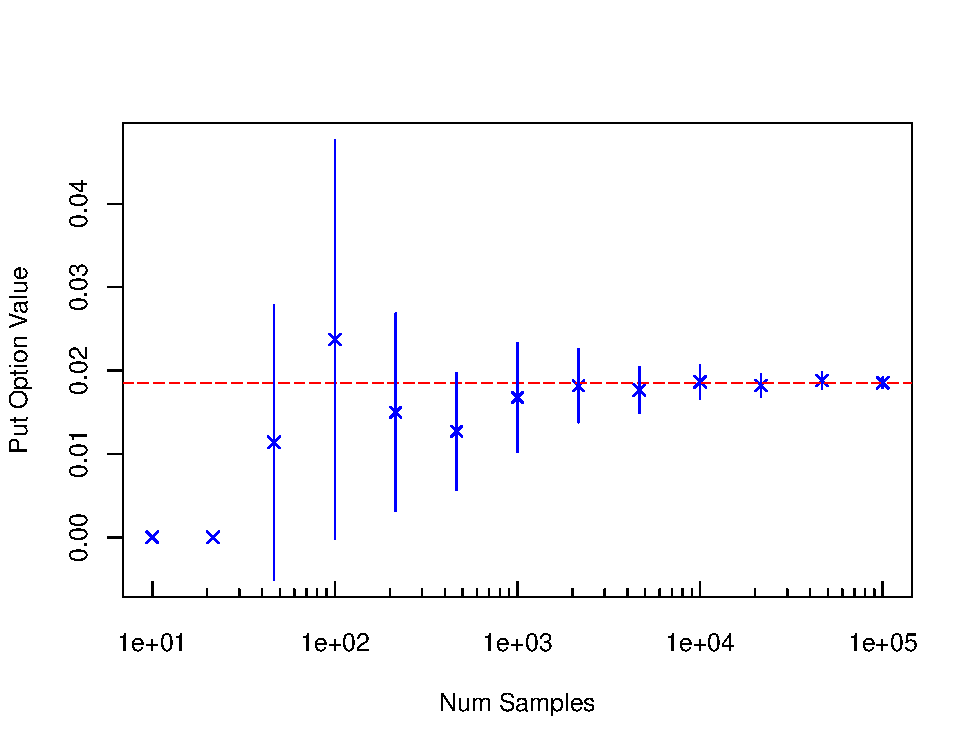
\includegraphics{./plots/putapprox.pdf}
\caption{Sample means and confidence intervals for an increasing number of simulations of a vanilla put option.}
\end{figure}

\indent At time $t > 0$ suppose the value of one share of a stock is $S(t)$. Assume that $S(t)$ follows a log-normal distribution (under the risk neutral probability measure) with mean
\begin{equation*}
	\ln S(0) + (r - \frac{1}{2}\sigma^2) t
\end{equation*}

and variance $\sigma^2 t$, where we say that $\sigma$ is the volatility of the stock and $r$ the risk free interest rate. For $t_j = j\frac{T}{s}$ we may compute the price at $S(t_j)$ using the recursive relationship
\begin{equation*}
	S(t_j) = S(t_{j-1})e^{(r - \frac{1}{2}\sigma^2)\Delta_j + \sigma \sqrt{\Delta_j}Z_j} \quad j = 1,...,s
\end{equation*}

where $\Delta_j = (t_j - t_{j-1})$ and $Z_j$ are i.i.d $N(0,1)$ such that $\sqrt{\Delta_j}Z_j \sim W_{t_j} - W_{t_{j-1}} \sim N(0, \Delta_j)$.

\subsubsection{Down \& Out Call Options}

\indent The time 0 price of a {\em down \& out call option} with barrier $b$, strike $K$, and expiry $T$ is given by
\begin{equation*}
	C_{do,0} = \mathbb E[e^{-rT}\mathds{1}_{\tau (b) > T}(S(T) - K)^+]
\end{equation*}

where 
\begin{equation*}
	\tau (b) = \inf\{t_i: S(t_i) < b\}
\end{equation*}

is the first time in $\{t_1, t_2, ... , t_s\}$ that the price of the underlying asset dips below $b$, and understood to be $\infty$ if the price never dips below $b$ for all $t_i$. \\

\underline{Example}: \\

\indent Consider the crude Monte-Carlo pricing of down \& call option with $S_0 = 100, b = 95, K = 110, T = 1, \sigma = 0.2, r = 0.05$, and $s = 52$.

\begin{figure}[H]
	\centering
 	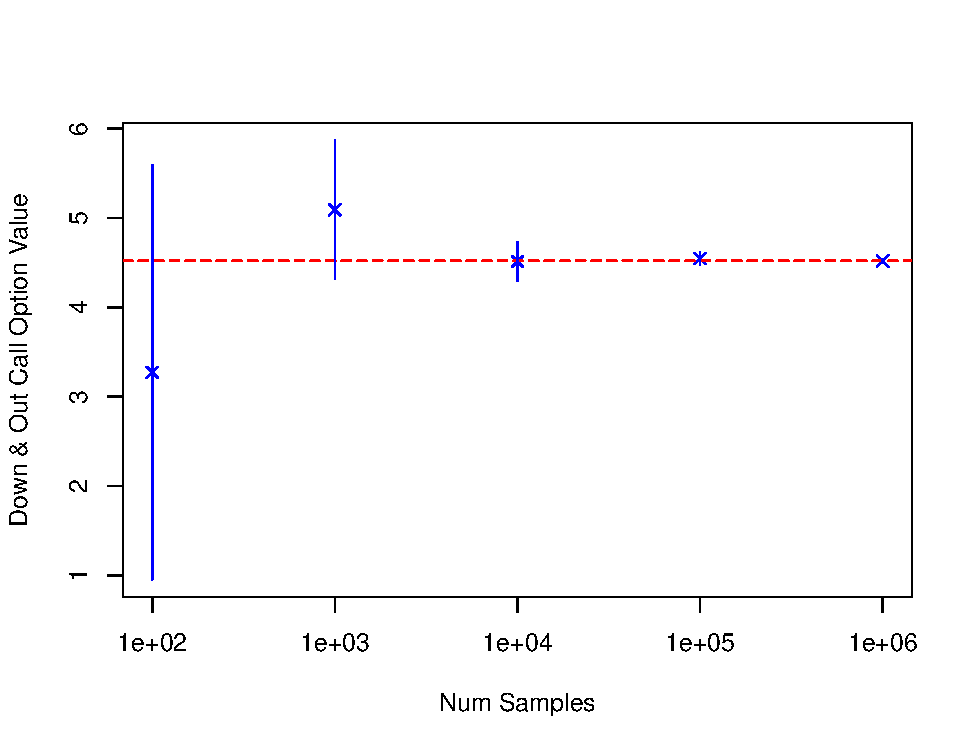
\includegraphics{./plots/d_o_callapprox.pdf}
\caption{Sample means and confidence intervals for an increasing number of simulations of a down \& out call option.}
\end{figure}

\subsection{Simulating an SDE -- Euler Discretization}

\indent We may simulate sample paths for a given model by discretizing its SDE with respect to time. For the SDE
\begin{equation*}
	r_t = r_0 + \int^t_0 \mu(u, r(u))\,du + \int^t_0 \sigma(u, r(u))\,dW_u
\end{equation*}

we consider a partition
\begin{equation*}
	0 = t_0 < t_1 < t_2 < \cdots < t_N = T
\end{equation*}

and as before let $\Delta t_j = \Delta t$ for all $t_j$. Then, the Euler discretization of the SDE is
\begin{align*}
	r_{t_{j+1}} - r_{t_j} &= \int^{t_{j+1}}_0 \mu(u, r(u))\,du + \int^{t_{j+1}}_0 \sigma(u, r(u))\,dW_u - \int^{t_{j}}_0 \mu(u, r(u))\,du - \int^{t_{j}}_0 \sigma(u, r(u))\,dW_u \\
	&= \int^{t_{j+1}}_{t_j} \mu(u, r(u))\,du + \int^{t_{j+1}}_{t_j} \sigma(u, r(u))\,dW_u \\
	&\approx \mu(t_j, r(t_j))\Delta t + \sigma(t_j, r(t_j))\Delta W_j
\end{align*}

where we have taken the left endpoint to match up with our definition of It\^{o} integrals. Depending on what function $\mu$ and $\sigma$ are, we can show that as $\Delta t \to 0$ such a discretization will converge (at least weakly, or in distribution, which is often sufficient) to the SDE solution.

\subsubsection{Forward-Starting Asian Call Option}

Suppose we have an underlying asset $S$ with price process under the risk neutral measure
\begin{equation*}
	S_t = S_0 + \int^t_0 rS_u\,du + \int^t_0 \sigma S_u\,dW_u
\end{equation*}

for $0 \leq t \leq T$. We are interested in pricing a forward-starting Asian call option with strike $K$. The time $T$ payoff is
\begin{equation*}
	\bigg(\frac{1}{n + 1} \sum^N_{j = 0} S_{s + j\Delta} - K\bigg)^+
\end{equation*}

where $s \geq 0$ is the time at which we begin calculating the average price, $\Delta$ is the monitoring frequency, and $N + 1$ is the number of dates used in computing the average price over the interval $[s, T]$. To price this derivative using Monte-Carlo methods we take $\Delta = (T - s)/N$ and partition $[s, T]$ by $\{s_j\}^N_{j=0}$ where $s_j = s + j\Delta$. We have a vector of dates $s = s_0, s_1, s_2, ..., s_N = T$ as the monitoring dates. We see that this is a path dependent option so we simulate the entire path and sample only the relevant dates. Given $S_0$ we have the solution to our SDE for $S_t$,
\begin{equation*}
	S_t = S_0 e^{(r - \frac{1}{2}\sigma^2)t + \sigma (B_t - B_0)}
\end{equation*}

Thus, the price at time $s_0 = s$ is
\begin{equation*}
	S_s = S_0 e^{(r - \frac{1}{2}\sigma^2)s + \sigma (B_s - B_0)}
\end{equation*} 

and the values of $S$ at times $\{s_j\}^N_{j = 1}$ as
\begin{equation*}
	S_{s_{j + 1}} = S_{s_j} e^{(r - \frac{1}{2}\sigma^2)\Delta + \sigma \big(B_{s_{j+1}} - B_{s_j}\big)}
\end{equation*}

\indent We may simulate these values by generating ${Z_j}^N{j=0}$ i.i.d $N(0,1)$ random variates and replacing the Brownian increments $B_s - B_0$ by $\sqrt{s}Z_0$ and $B_{s_{j+1}} - B_{s_j}$ by $\sqrt{s_{j+1} - s_j}Z_{j+1}$. Thus, we require $N + 1$ normal random variables to simulate our prices at each monitoring date
\begin{equation*}
	S_s = S_0, S_{s_1}, S_{s_2}, ..., S_{s_N} = S_T
\end{equation*}

to compute the option payoff. Thus, the time 0 value of this option is
\begin{equation*}
	C_0^{FwdAsianCall} = \mathbb E_{\mathbb Q}\bigg[e^{-rT} \bigg(\frac{1}{N+1}\sum^{N}_{j=0} S_{s + j\Delta} - K \bigg)^+ \bigg]
\end{equation*}

which may be estimated using crude estimators by
\begin{equation*}
	\hat{C_0}^{FwdAsianCall} = \frac{1}{M}e^{-rT} \sum^M_{i=1} \big(FwdAsianAvg(r,\sigma,S_0,S,T,Z_i) - K\big)^+
\end{equation*}

\section{Variance Reduction}

\indent Variance reduction techniques sometimes affords us efficiency gains, allowing us to compute fewer samples for the same amount of accuracy, or greater accuracy for the same number of samples.

\subsection{Crude Estimators}

Given the estimator
\begin{equation*}
	\theta = \mathbb E[f(U)] = \mathbb E[g(X)]
\end{equation*}

we say that
\begin{equation*}
	\hat{\Theta}_{CR} = \frac{1}{N}\sum^{N}_{i=1} f(U_i)
\end{equation*}

is the crude Monte-Carlo estimator for $\theta$. We know that $\hat{\Theta}_{CR}$ is unbiased:
\begin{equation*}
	\mathbb E[\hat{\Theta}_{CR}] = \theta
\end{equation*}

and has variance
\begin{equation*}
	\mathrm{Var}[\hat{\Theta}_{CR}] = \frac{1}{N}\mathrm{Var}[f(U_i)] = \frac{\sigma^2}{N}
\end{equation*}

\indent Notice that for $N\to\infty$ we have $\mathrm{Var}[\hat{\Theta}_{CR}] \to 0$, which is nice, but is sometimes not fast enough for our purposes.

\begin{definition} The \underline{efficiency} of an estimator $\hat{\theta}$ for a parameter $\theta$, denoted $\mathrm{Eff}[\hat{\theta}]$, is
\begin{equation*}
	\mathrm{Eff}[\hat{\theta}] = \frac{1}{\mathrm{MSE}[\hat{\Theta}] \cdot C[\hat{\theta}]}
\end{equation*}

where
\begin{align*}
	\mathrm{MSE}[\hat{\theta}] &= \mathrm{Var}[\hat{\theta}] + \mathrm{Bias}^2[\hat{\theta}] \\
	\mathrm{Bias}[\hat{\theta}] &= \mathbb E[\hat{\theta} - \theta] = \mathbb E[\hat{\theta}] - \theta \\
	C[\hat{\theta}] &= \text{Expected computation time of } \hat{\theta}\\
\end{align*}

We say that the larger the efficiency, the better the estimator is.
\end{definition}

\indent Suppose $\hat{\theta}_1, \hat{\theta}_2$ are both unbiased estimators for $\theta$ and $C[\hat{\theta}_1] = C[\hat{\theta}_2]$, then we prefer $\hat{\theta}_1$ over $\hat{\theta}_2$ if
\begin{equation*}
	\mathrm{Var}[\hat{\theta}_1] < \mathrm{Var}[\hat{\theta}_2]
\end{equation*}

\indent Suppose the computation time for the crude estimator $\hat{\Theta}_{CR}$ based on $n$ samples of $U\sim Unif(0,1)$ is $c\cdot n$ for some constant $c > 0$. Since $\hat{\Theta}_{CR}$ is unbiased
\begin{align*}
	\mathrm{Eff}[\hat{\Theta}_{CR}] &= \frac{1}{\mathrm{MSE}[\hat{\Theta}_{CR}] \cdot C[\hat{\Theta}_{CR}]} \\
	&= \frac{1}{(\mathrm{Var}[\hat{\Theta}_{CR}] + \mathrm{Bias}^2[\hat{\Theta}_{CR}])\cdot C[\hat{\Theta}_{CR}]} \\
	&= \frac{1}{\mathrm{Var}[\hat{\Theta}_{CR}]\cdot C[\hat{\Theta}_{CR}]} \\  
	&= \frac{1}{\frac{\sigma^2}{n}\cdot (c\cdot n)} \\
	&= \frac{1}{c\sigma^2}
\end{align*}

which we see is independent of $n$. Therefore, efficiency gain afforded by the decrease in variance is exactly offset by the loss of efficiency afforded increased computation time for an additional number of samples. Our goal is to now find more efficiency estimators than $\hat{\Theta}_{CR}$ that reduce variance more quickly than the increase in computation time.

\subsection{Antithetic Variates}

\indent The idea underlying antithetic variables is to use negatively correlated pairs of variates in estimating our parameter. We expect that the negative correlation between the pairs should cancel out the variation from $\theta$, or at least some of the variation, if not a perfect negative correlation. Assume $n$ even and let $Y = h(X)$ and $\mathbb E[Y] = \theta$. Let the pairs
\begin{equation*}
	(Y_1, \overline{Y}_2), (Y_2, \overline{Y}_2), ... , (Y_{n/2}, \overline{Y}_{n/2})
\end{equation*}

be $n/2$ i.i.d. \underline{antithetic} pairs. We require $Y_i, \overline{Y}_i$ to have a negative correlation, and pairs $(Y_i, \overline{Y}_i), (Y_j, \overline{Y}_j)$ should be independent, for $i \neq j$. Then, the antithetic estimator $\hat{\Theta}_{AT}$ for $\theta = \mathbb E[Y]$ is
\begin{equation*}
	\hat{\Theta}_{AT} = \frac{1}{n/2} \sum^{n/2}_{i=1} \bigg(\frac{Y_i + \overline{Y}_i}{2}\bigg)
\end{equation*} 

\begin{theorem}{Some results for antithetic estimators} For an antithetic estimator $\hat{\Theta}_{AT}$ based on $n/2$ pairs of variates, we have
\begin{align*}
	\mathbb E[\hat{\Theta}_{AT}] &= \theta \\
	\mathrm{Var}[\hat{\Theta}_{AT}] &= \frac{\sigma^2}{n} + \frac{1}{n}\mathrm{Cov}[Y_i, \overline{Y}_i] \\
	&< \frac{\sigma^2}{n} = \mathrm{Var}[\hat{\Theta}_{AT}] \quad \text{if } \mathrm{Cov}[Y_i, \overline{Y}_i] < 0
\end{align*}
\end{theorem}

\indent If we have $\mathrm{Cov}[Y_i, \overline{Y}_i] = -\mathrm{Var}[Y_i]$ then the antithetic estimator works perfectly (i.e. no variance). In general, it is difficult to induce a perfect negative correlation between $Y_i$ and $\overline{Y}_i$ since we rarely generate them directly and instead are generated as a function of uniform/normal variates. The general method for applying antithetic variables is
\begin{align*}
	Y_i &= f(U_{i_1}, U_{i_2}, ..., U_{i_m}) \\
	\overline{Y}_i &= f(1 - U_{i_1}, 1 - U_{i_2}, ..., 1 - U_{i_m})
\end{align*}

\begin{theorem}{Minimum correlation between random variables} If $X$ is a random variable with cdf $F$ and $\overline{U} = 1 - U$, where $U\sim Unif(0,1)$, then $(F^{-1}(U), F^{-1}(\overline{U}))$ has the minimum correlation among all pairs of random variables with cdf $F$.
\end{theorem}

\indent Usually we are interested in the expectation of a function of a random variable $h(X)$, rather than the pure expectation of the random variable itself. The above theorem is not always useful/applicable in these cases since it may not specify the minimum correlation.

\begin{theorem}{Covariance of monotone functions of antithetic variables} Let $f: [0,1)^s \to \mathbb R$ be a bounded monotonic function in each of its $s$ arguments. Suppose that $f$ is not constant on the interior of its domain. Then,
\begin{equation*}
	\mathrm{Cov}[f(U_1, U_2, ..., U_s), f(1 - U_1, 1 - U_2, ..., 1 - U_s)] < 0 
\end{equation*}
\end{theorem}

\indent In practice, these conditions (i.e. monotonicity/boundedness) are difficult to verify. However, if they are satisfied then we are guaranteed a smaller variance for the antithetic estimator than the crude Monte-Carlo estimator. \\

\underline{Example}: Suppose $F$ is the cdf of a normal random variable with mean $\mu$ and variance $\sigma^2$. We can prove that
\begin{equation*}
	F^{-1}(1 - U) = 2\mu - F^{-1}(U)
\end{equation*}

\indent Thus, to produce two antithetic normal random variables $X_1, \overline{X}_1$, it is equivalent to generate $X_1 \sim N(\mu,\sigma^2)$ and set
\begin{equation*}
	\overline{X}_1 = 2\mu - X_1
\end{equation*}

\indent That is, to generate two normal random variables it is not necessary to use the inverse transform method with antithetic uniform variates.

\subsection{Control Variates}

We may estimate the integral
\begin{equation*}
	\theta = \int^1_0 f(u)\,du
\end{equation*}

with the crude estimator
\begin{equation*}
	\hat{\Theta}_{CR} = \frac{1}{n} \sum^n_{i=1} f(U_i)
\end{equation*}

for $U_i$ i.i.d. $Unif(0,1)$ variables. Suppose that we have some function $g$ such that $f(U_i)$ and $g(U_i)$ are positively correlated, and suppose that we can compute
\begin{equation*}
	\theta_g = \mathbb E[g(U)]
\end{equation*}

exactly (i.e. without estimation). If the crude estimator of $\theta_g$ is $\hat{\Theta}_g$ such that
\begin{equation*}
	\hat{\Theta}_g = \frac{1}{n} \sum^n_{i=1} g(U_i)
\end{equation*}

is larger than $\theta_g$ then, on average, $\hat{\Theta}_{CR}$ is also probably larger than $\theta$. The idea will be to adjust the crude estimator $\hat{\Theta}_{CR}$ by subtracting some positive value related to the magnitude of $\hat{\Theta}_g - \theta_g$, and if $\hat{\Theta}_g < \theta_g$ then we should add some positive value to $\hat{\Theta}_{CR}$.

\begin{definition} A \underline{control variate estimator} is an estimator of the form
\begin{align*}
	\hat{\Theta}_{CV} &= \frac{1}{n} \sum^n_{i=1} \Big[f(U_i) + \beta \big(\theta_g - g(U_i)\big) \Big] \\
	&= \frac{1}{n} \sum^n_{i=1} \Big[f(U_i) - \beta \big(g(U_i) - \mathbb E[g(U_i)]\big)\Big]
\end{align*}

where $\beta$ is some constant.
\end{definition}

\begin{proposition} The control variate estimator $\hat{\Theta}_{CV}$ is unbiased.
\end{proposition}

\indent In general, we see to find a constant $\beta$ such that the variance of the control variate estimator is minimized. It turns out that the value the optimal $\beta$, denoted $\beta^*$, is
\begin{equation*}
	\beta^* = \frac{\mathrm{Cov}[f(U_i),g(U_i)]}{\mathrm{Var}[g(U_i)]}
\end{equation*}

So, in this case\footnote{Which case is this again? I think it was the expected value?} we have
\begin{equation*}
	\mathrm{Var}[\hat{\Theta}_{CV}] = (1 - \rho^2)\mathrm{Var}[\hat{\Theta}_{CR}]
\end{equation*}

where $-1 \leq \rho \leq 1$ is the correlation coefficient between $f(U_i)$ and $g(U_i)$
\begin{equation*}
	\rho = \frac{\mathrm{Cov}[f(U_i),g(U_i)]}{\sqrt{\mathrm{Var}[f(U_i)]\mathrm{Var}[g(U_i)]}}
\end{equation*}

\indent Unfortunately for us, $\mathrm{Cov}[f(U_i), g(U_i)]$ is usually unknown. If it was known then $\theta$ would be known and there'd be no point to computing a Monte-Carlo estimator! We can estimate $\beta^*$ by replacing the unknown quantities with their standard estimators
\begin{equation*}
	\hat{\beta}^* = \frac{\sum^n_{i=1}\big(f(U_i)g(U_i)\big) - n\hat{\Theta}_{CR}\hat{\Theta}_g }{(n-1)s^2_g}
\end{equation*}

where
\begin{equation*}
	s^2_g = \frac{1}{n-1} \sum^n_{i=1} \Big(g(U_i) - \hat{\Theta}_{g} \Big)^2
\end{equation*}

is the sample variance. If $\mathrm{Var}[g(U_i)]$ is known then we may just replace it with $s^2_g$ in the estimator for $\beta^*$. The drawback with the estimator $\hat{\beta}^*$ is that the new control variate estimator for $\theta$,
\begin{equation*}
	\hat{\Theta}_{CR,\hat{\beta}^*} = \hat{\Theta}_{CR} + \hat{\beta}^*(\theta_g - \hat{\Theta}_g)
\end{equation*}

is no longer necessarily unbiased, though it can be shown that it is asymptotically unbiased as $n \to \infty$. Furthermore, the expression we have found for the variance of the control variate estimator
\begin{equation*}
	\mathrm{Var}[\hat{\Theta}_{CR}] = (1 - \rho^2)\mathrm{Var}[\hat{\Theta}_{CR}]
\end{equation*}

no longer holds when using the estimator $\hat{\beta}^*$ for $\beta$. That is, we cannot use this relationship to get an idea of the variance of our estimator. Even the standard sample variance estimator is no longer unbiased when using $\hat{\beta}^*$! \\

\subsubsection{Pilot Runs \& Control Variates}

\indent An alternative approach to the control variate technique is to use a different sample (i.e. a pilot sample) $(U_1, U_2, ..., U_m)$ to first estimate $\hat{\beta}^*$. Once $\hat{\beta}^*$ is computed we then generate $(U_{m+1}, ... U_{n+m})$, independent of the first $m$ variables, to compute $\hat{\Theta}_{CR,\hat{\beta}^*}$. In general, note that
\begin{enumerate}
	\item We require $n > m$
	\item The estimator $\hat{\beta}^*$ is calculated independent of $\hat{\Theta}_g$ so that the control variate estimator is unbiased 
	\item We have the drawback of additional effort/simulation
\end{enumerate}

\indent In principle it is possible to use multiple control variates and keep track of each with vector notation. However, additional control variates are not {\em ipso facto} better since we would need to estimate the optimal vector valued $\vec{\beta}$ and including additional components to the estimator introduces additional noise to the overall estimator. \\

\subsubsection{Which Control Variate to Use?}

\indent In general, nobody is going to tell you exactly which control variate to use/which control variate is optimal. In theory, we may choose any function $g$ such that $f(U)$ and $g(U)$ are uncorrelated, and $g(U)$ has the known expectation $\mathbb E[g(U)]$. We also look for a function $g$ related to $f$ but is simpler to compute. \\

\indent The function $g$ could also be the same as $f$ but for a simpler model than $f$. For example, suppose we were interested in estimating the mean waiting time in a complicated queueing system. We could first using the mean waiting time of a simpler system with some relationship to the complicated system. For this to work we require some correlation between the systems represented by $f$ and $g$. \underline{Synchronization}: Use the same uniform random variables to generate the inter-arrival \& service times in both models.

\subsection{Importance Sampling}

\indent Importance sampling is a variance reduction technique not related to the manipulation of correlated sampling. Instead, the idea is to ``focus'' the sampling effort to the ``most important region'' for the simulation problem more often than would be done in other sampling techniques. This technique is most useful when trying to estimate rare events that often result in extremely high variance estimators (i.e. VaR, Bankruptcy, pricing extremely OTM derivatives, etc...). \\

\indent The idea is similar to the change probability distribution (change of measure) of vector valued random variable $\vec{X}$ to generated values in which the rare event(s) is (are) more likely to occur. \\

\indent Suppose $\vec{X}$ taking on values $\vec{x}\in\mathbb R^d$ has density $\phi(\vec{x})$ (or measure $dP(\omega) = \phi(\vec{x})\,d\vec{x})$. We wish to estimate
\begin{equation*}
	\mu = \mathbb E_{\phi}[h(\vec{X})] = \int_{\mathbb R^d} h(\vec{x})\phi(\vec{x})\,d\vec{x} = \int_\Omega h(\vec{X}(\omega))\,dP(\omega)
\end{equation*}

\indent To do so we use an alternate density (measure) for $\vec{X}$ with density $\psi(\vec{x})$ (or measure $d\overline{P}(\omega) = \psi(\vec{x})\,d\vec{x}$). We write
\begin{equation*}
	\mu = \int_{\mathbb R^d} h(\vec{x})\phi(\vec{x})\frac{\psi(\vec{x})}{\psi(\vec{x})} = \int_{\mathbb R^d} h(\vec{x})L(\vec{x})\psi(\vec{x})\,d\vec{x}
\end{equation*}

where $L(\vec{x}) = \frac{\phi(\vec{x})}{\psi(\vec{x})}$ is the likelihood ratio. For crude Monte-Carlo estimation we have the estimator
\begin{equation*}
	\hat{\mu}_{CR} = \frac{1}{n} \sum^n_{i=1} h(\vec{X}_i)
\end{equation*}

where $\vec{X}_i$ is drawn from the density $\phi(\vec{x})$. Instead, using importance sampling, we generate a random sample $\vec{Y}_i$ drawn from the density $\psi(\vec{x})$ and use the estimator
\begin{equation*}
	\hat{\mu}_{IS} = \frac{1}{n} \sum^n_{i=1} h(\vec{Y}_i)L(\vec{Y}_i)
\end{equation*}

\indent We call $\hat{\mu}_{IS}$ the \underline{importance sampling estimator} of $\mu$. In order to ensure that the likelihood ratio $L(\vec{x})$ is well defined (i.e. no division by zero) we require that $\phi(\vec{x}) = 0$ for all $\vec{x} \in \mathbb R^d$ such that $\psi(\vec{x}) = 0$ and let $L(\vec{x}) = 0$ for these values of $\vec{x}$. This is equivalent to when we were manipulating the real-world measure to the risk neutral measure. In effect, we ensured that a measure $\mathbb P$ is absolutely continuous with respect to $\mathbb {\overline{P}}$. This ensures that the Radon-Nikodym density of $\mathbb P$ with respect to $\mathbb {\overline{P}}$ is well defined.

\begin{theorem}{The importance sampling estimator is unbiased} \hfill
\begin{proof} We note
\begin{align*}
	\mathbb E_{\psi}[\hat{\mu}_{IS}] = \frac{1}{n} \sum^n_{i=1} \mathbb E_{\psi}[h(\vec{Y}_i)L(\vec{Y}_i)] &= \frac{1}{n} \sum^n_{i=1} \int_{\mathbb R^d} h(\vec{y}_i)L(\vec{y}_i) \psi(\vec{y}_i)\,d\vec{y}_i \\
	&= \int_{\mathbb R^d} h(\vec{y}) \frac{\phi(\vec{y})}{\psi(\vec{y})}  \psi(\vec{y})\,d\vec{y} \\
	&= \int_{\mathbb R^d} h(\vec{y}) \phi(\vec{y}) \,d\vec{y} \\
	&= \mu
\end{align*}
\end{proof}
\end{theorem}

\indent Note that not all selections of $\psi(x)$ will necessarily reduce the variance of the estimator with respect to the crude estimator. Consider
\begin{align*}
	\mathbb E_{\psi}[h^2(\vec{Y})L^2(\vec{Y})] &= \int h^2(\vec{y})L^2(\vec{y}) \psi(\vec{y}) \,d\vec{y} \\
	&= \int h^2(\vec{y}) \frac{\phi^2(\vec{y})}{\psi^2(\vec{y})} \psi(\vec{y}) \,d\vec{y} \\
	&= \int h^2(\vec{y}) \frac{\phi^2(\vec{y})}{\psi(\vec{y})} \,d\vec{y} \\
	&= \int h^2(\vec{y}) \frac{\phi(\vec{y})}{\psi(\vec{y})} \phi(\vec{y}) \,d\vec{y} \\
	&= \mathbb E_{\phi}[h^2(\vec{Y})L(\vec{Y})] \\
	\implies \mathrm{Var}_{\psi}[\hat{\mu}_{IS}] &= \frac{1}{n}\bigg( E_{\phi}[h^2(\vec{Y})L(\vec{Y})] - \mu^2 \bigg)
\end{align*} 

Thus, the variance of the importance sampling estimator is reduced if and only if
\begin{equation*}
	E_{\phi}[h^2(\vec{Y})L(\vec{Y})] < \mathbb E_{\phi}[h^2(\vec{Y})]
\end{equation*}

\indent That is, if $L(\vec{y}) < 1$ whenever $h(\vec{y}) \neq 0$, which is rarely verifiable in practice. We note that $L(\vec{y}) < 1$ means that $\vec{y}$ is more likely. Thus, when $h(\vec{y})$ is large the new pdf should make $\vec{y}$ more likely to that $L(\vec{y})$ is now small. When $h(\vec{y})$ is small we can afford to have $L(\vec{y}) > 1$. In practice, there is no general good method to pick a new density. We often pick a new density $\psi(x)$ so that $X_i$ has the same distribution as $phi(x)$ but with different parameters.












\end{document}